\documentclass{article}
\usepackage[ngerman]{babel}
\usepackage[utf8]{inputenc}
\usepackage{fancyhdr}
\usepackage{libertine} 
\usepackage{dirtree}
\usepackage{float}
\usepackage{minted}
\usepackage{graphicx}
\usepackage[hyphens]{url}
\usepackage{listings}
\usepackage{booktabs}

\pagestyle{fancy}

\renewcommand{\headrulewidth}{0.4pt}
\renewcommand{\footrulewidth}{0.4pt}
\cfoot{Seite \thepage}

\title{Das Django Webframework am Beispieles eines Inventarisierungssystemes}
\author{Clemens Dautermann}
\date{2. Januar 2019 bis \today}

\lstset{literate=
	{á}{{\'a}}1 {é}{{\'e}}1 {í}{{\'i}}1 {ó}{{\'o}}1 {ú}{{\'u}}1
	{Á}{{\'A}}1 {É}{{\'E}}1 {Í}{{\'I}}1 {Ó}{{\'O}}1 {Ú}{{\'U}}1
	{à}{{\`a}}1 {è}{{\`e}}1 {ì}{{\`i}}1 {ò}{{\`o}}1 {ù}{{\`u}}1
	{À}{{\`A}}1 {È}{{\'E}}1 {Ì}{{\`I}}1 {Ò}{{\`O}}1 {Ù}{{\`U}}1
	{ä}{{\"a}}1 {ë}{{\"e}}1 {ï}{{\"i}}1 {ö}{{\"o}}1 {ü}{{\"u}}1
	{Ä}{{\"A}}1 {Ë}{{\"E}}1 {Ï}{{\"I}}1 {Ö}{{\"O}}1 {Ü}{{\"U}}1
	{â}{{\^a}}1 {ê}{{\^e}}1 {î}{{\^i}}1 {ô}{{\^o}}1 {û}{{\^u}}1
	{Â}{{\^A}}1 {Ê}{{\^E}}1 {Î}{{\^I}}1 {Ô}{{\^O}}1 {Û}{{\^U}}1
	{Ã}{{\~A}}1 {ã}{{\~a}}1 {Õ}{{\~O}}1 {õ}{{\~o}}1
	{œ}{{\oe}}1 {Œ}{{\OE}}1 {æ}{{\ae}}1 {Æ}{{\AE}}1 {ß}{{\ss}}1
	{ű}{{\H{u}}}1 {Ű}{{\H{U}}}1 {ő}{{\H{o}}}1 {Ő}{{\H{O}}}1
	{ç}{{\c c}}1 {Ç}{{\c C}}1 {ø}{{\o}}1 {å}{{\r a}}1 {Å}{{\r A}}1
	{€}{{\euro}}1 {£}{{\pounds}}1 {«}{{\guillemotleft}}1
	{»}{{\guillemotright}}1 {ñ}{{\~n}}1 {Ñ}{{\~N}}1 {¿}{{?`}}1
}

\begin{document}

\maketitle
\newpage
\tableofcontents
\newpage


\section{Einleitung}
Diese Facharbeit soll einen grundlegenden Überblick über die wichtigsten Funktionen des Django Web-Frameworks geben.\newline
Das Django Web-Framework ist ein größtenteils in Python geschriebenes\footnote{Offizielle Django GitHub Seite https://github.com/django/django} Framework
zum entwickeln von Webservern. Es ist aufgrund seiner ausgeprägten Modularität und der Existenz einer Vielzahl von Datenbanktreibern besonders gut für
die Entwicklung von Webservern geeignet, die eine Datenbank erfordern.\newline 
Django stellt eine grundlegende Struktur für die Entwicklung zur Verfügung. So zum Beispiel:
\begin{itemize}
	\item Eine settings.py Die genutzt werden kann um Konfigurationsmöglichkeiten zentral zu bündeln
	\item Eine library um einfache Zugriffe auf Datenbanken zu tätigen und sogenannte Models um Datenbankobjekte zu verwalten
	\item Ein Routingsystem um eine einfachere Verwaltung von Urls zu gewährleisten
	\item Eine Grundstruktur, die Modularität unterstützt und das einfache Installieren oder Entfernen von sogenannten ''Apps'' ermöglicht
\end{itemize}
Es ist also kaum notwendig, jedoch durchaus möglich, als Entwickler noch SQL zu schreiben wenn man mit dem Django Web-Framework entwickelt.
\section{Struktur}
Ein typischer Django Server ist aus sogenannten ''Apps'' aufgebaut. Diese werden entweder vom Entwickler selber geschrieben oder können via pip (dem Python Paket Manager) installiert werden. Ein standard Verzeichnisaufbau ist in Abbildung 1 dargestellt.
\begin{figure}[H]
	\dirtree{%
		.1 server.
		.2 manage.py.
		.2 db.sqlite3.
		.2 server.
		.3 \_\_init\_\_.py.
		.3 settings.py.
		.3 urls.py.
		.3 wsgi.py.
		.2 app1.
		.3 \_\_init\_\_.py.
		.3 admin.py.
		.3 apps.py.
		.3 forms.py.
		.3 models.py.
		.3 tests.py.
		.3 urls.py.
		.3 views.py.
		.3 migrations.
		.4 0001\_initial.py.
	}
	\caption{Die typische Verzeichnisstruktur eines Django Servers}
\end{figure}

\subsection{Erstellung}
Ein Django Projekt kann mit dem Befehl \$ django-admin startproject server initialisiert werden. Dadurch wird folgende Ordnerstruktur erstellt:
\begin{figure}[H]
	\dirtree{%
	.1 server.
	.2 manage.py.
	.2 server.
	.3 \_\_init\_\_.py.
	.3 settings.py.
	.3 urls.py.
	.3 wsgi.py.
}
\caption{Verzeichnisstruktur, die der \$ django-admin startproject server Befehl erzeugt}
\end{figure}
\subsection{manage.py}
Die manage.py wird, wie der Name schon sagt, verwendet um den Server zu verwalten. Mit Hilfe der manage.py können beispielsweise Migrierungen an der Datenbank erstellt werden, Datenbanknutzer erstellt werden oder der Testserver zur Entwicklung kann gestartet werden. Die gleiche Funktionalität stellt auch der django-admin Befehl zur Verfügung\footnote{Django Dokumentation https://docs.djangoproject.com/en/2.1/ref/django-admin/}.

\subsection{db.sqlite3}
In dieser Datei wird die SQL Datenbank gespeichert, die der Server nutzt. Sie wird automatisch erstellt. Es können jedoch auch andere Datenbanken, wie zum Beispiel MongoDB oder eine extern gehostete Datenbank, verwendet werden.

\subsection{server/server} 
\subsubsection{\_\_init\_\_.py}
Diese Datei befindet sich im Wurzelverzeichnis jeder App. Sie macht für Python erkennbar, dass es sich bei dem Inhalt dieses Ordners um ein Python Modul handelt. Somit kann die App einfach geteilt und von anderen Nutzern verwendet werden.[linenos, frame=lines, framesep=2mm]{Python}

\subsubsection{settings.py}
In dieser Datei befinden sich die Einstellungen für den Django Server. Mit ihrer Hilfe werden Zeitzone, Sprache, Datenbankkonfiguration und viele andere Konfigurationen verwaltet. Man kann sie auch verwenden um eigene Einstellungsmöglichkeiten anzubieten. Dafür definiert man eine Konstante (in Python typischerweise durch Großbuchstaben ausgedrückt) und einen Wert. Zum Beispiel\newline LOGIN\_REDIRECT\_URL = ''/''. Im Falle dieses Projektes wurde beispielsweise die Konstante LOGFILE = 'serverlog.log' definiert um zentral auf die Logdatei zugreifen zu können. Auf die in der settings.py definierten Werte kann aus jeder App zugegriffen werden, indem unter Benutzung der Anweisung\newline
 \mintinline{Python}{from django.conf import settings }  diese importiert wird. Anschließend kann via \mintinline{Python}{file = settings.LOGFILE} beispielsweise auf die Konstante LOGFILE zugegriffen werden.
 
\subsubsection{urls.py}
Diese Datei ist der erste und wichtigste Teil des Django Routing Systems. Über sie werden die grundlegenden URL Strukturen des Servers definiert. Sie importiert urls.py Dateien aus anderen Apps und definiert wie auf eine Bestimmte URL reagiert werden soll. Im Falle dieses Projektes sieht sie folgendermaßen aus:

\begin{minted}[linenos,numbersep=5pt,frame=none,framesep=2mm]{Python}
from django.contrib import admin
from django.urls import path, include
	
urlpatterns = [
path('admin/', admin.site.urls),
path('accounts/', include('django.contrib.auth.urls')),
path('', include('user_manager.urls')),
path('add/', include('object_adder.urls')),
path('list/', include('object_lister.urls')),
path('settings/', include('settings_app.urls')),
]
\end{minted}
Hier werden zuerst Pakete für das admin-Interface und Pakete für das URL-Routing importiert. Anschließend wird eine Liste urlpatterns definiert. Diese enthält alle URL Pfade. include() Importiert dabei die urls.py Dateien aus den anderen apps.

\subsubsection{wsgi.py}
Diese Datei stellt ein ''application'' genanntes WSGI Objekt zur Verfügung. Es wird zum starten des Testservers genutzt. In Verbindung mit ''mod\_wsgi'' kann auch Apache dieses Objekt nutzen.\footnote{Django Dokumentation https://docs.djangoproject.com/en/2.1/howto/deployment/wsgi/}
\subsection{server/app1}
Dieses Verzeichnis enthält alle Dateien, die eine App ausmachen. In diesem Fall heißt die App beispielhaft ''app1''. Die Dateien, die in Abb 1 erscheinen, jedoch hier nicht erwähnt werden, haben die selbe Funktion wie die gleichnamigen Dateien im ''server/server'' Ordner.

\subsubsection{admin.py}
Die admin.py dient dazu das Django Admin Interface zu konfigurieren. In ihr werden die Models registriert, die auf der admin Seite zu sehen sind, und wie diese dargestellt werden sollen. Sie sieht beispielsweise in der ''object\_adder'' app folgendermaßen aus:

\begin{minted}[linenos, frame=lines, framesep=2mm]{Python}
from django.contrib import admin
from .models import Object, Category


class ObjectAdmin(admin.ModelAdmin):
	list_display = ('title', 'ammout', 'uuid', 'img')


class CategoryAdmin(admin.ModelAdmin):
	list_display = ('name', 'id')


# Register your models here.
admin.site.register(Object, ObjectAdmin)
admin.site.register(Category, CategoryAdmin)
\end{minted}
In Zeile 2 werden die in der models.py definierten Models importiert um Zugriff auf diese zu erlangen.
\newline
Anschließend wird für jedes Model eine Klasse erstellt. In dieser Klasse wird jeweils eine ''list\_display'' Variable definiert, die ein Tupel enthält, mit dem alle darzustellenden Attribute an die admin library übergeben werden können. Diese Abmin-Klassen müssen jetzt noch zusammen mit dem Model an die admin library übergeben werden. Dies erfolgt duch die Befehle in Zeile 14 und 15. Dieser Code erzeugt demnach folgendes Admin-Interface:
\newline
\begin{center}
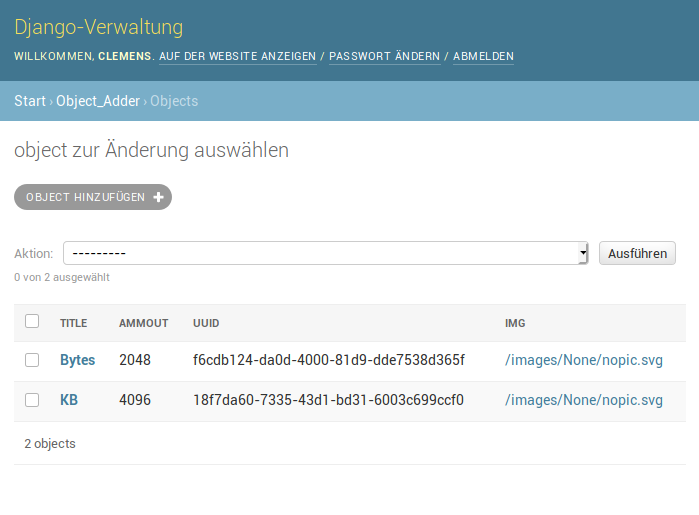
\includegraphics[width=\linewidth, height=7.5cm]{django_admin_objects.png}
\quad
\\[\baselineskip]% adds vertical line spacing
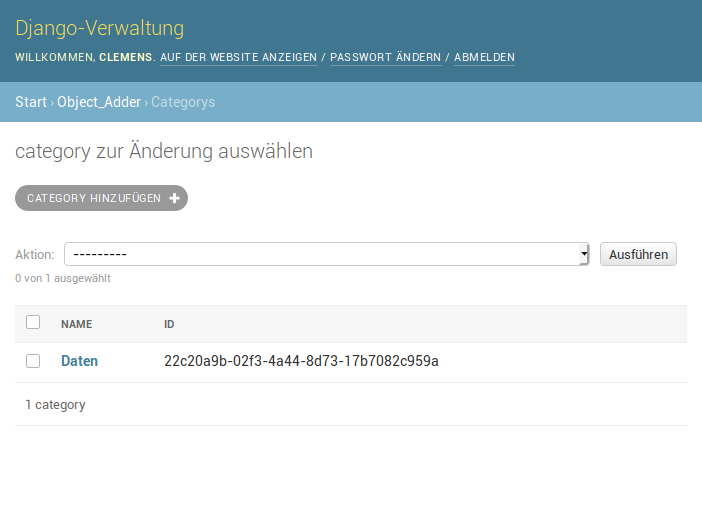
\includegraphics[width=\linewidth]{django_admin_cats.png}
\end{center}

Ohne die ''list\_display'' Angebe würde nur der primary key des Models angezeigt und das Interface sähe folgendermaßen aus:
\newline
\begin{center}
	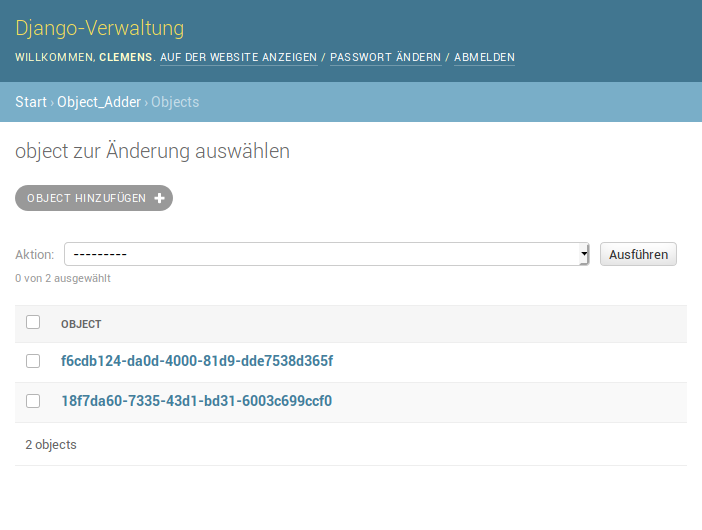
\includegraphics[width=\linewidth]{django_admin_obj_pk.png}
\end{center}
\subsubsection{apps.py}
Hier ist der Name der app definiert. Diese Datei ist außerdem notwendig, damit die App von Django als solche erkannt wird.
\begin{minted}[linenos, frame=lines, framesep=2mm]{Python}
from django.apps import AppConfig

class ObjectAdderConfig(AppConfig):
	name = 'objectadder'
\end{minted}
\subsubsection{forms.py}
In dieser Datei werden Formulare definiert. So beispielsweise das Formular zur Erstellung von Objekten und Kategorien, das folgendermaßen aussieht:
\begin{minted}[linenos, frame=lines, framesep=2mm]{Python}
from django.forms import ModelForm, TextInput	
from .models import Object, Category
	
	
class ObjectForm(ModelForm):
	class Meta:
		model = Object
		fields = ('ammout', 'title', 'img', 
		'description', 'category')
		widgets = {
			'title': TextInput(),
		}
	
	
class CategoryForm(ModelForm):
	class Meta:
		model = Category
		fields = ['name']
		widgets = {
			'name': TextInput()
		}
\end{minted}
Hier werden zwei Formulare definiert. Es wird angegeben mit welchem model das Formular asoziiert werden soll und welche Felder angezeigt werden sollen. Außerdem wird definiert, dass für das name und das title Feld ein ''TextInput()'' Feld genutzt werden soll.
\subsubsection{models.py}
In der models.py werden Models definiert, die in Verbindung mit der Datenbank genutzt werden können. Diese werden innerhalb von Django als Objekte repräsentiert, können jedoch trotzdem in einer SQL Datenbank gespeichert werden. Eine models.py kann beispielsweise folgendermaßen aussehen:
\begin{minted}[linenos, frame=lines, framesep=2mm]{Python}
from django.db import models
import uuid

	class Category(models.Model):
		name = models.TextField(blank=False, max_length=150)
		id = models.UUIDField(
		primary_key=True, default=uuid.uuid4, editable=False
		)	
		categories = models.Manager()
		
		def __str__(self):
			return self.name
	
\end{minted}
In dieser Datei wird ein Model definiert. Es heißt ''Category'' und hat zwei Eigenschaften. Eine ID und einen Namen. Es wird dafür erst eine Klasse namens ''Category'' erstellt, die Subklasse der django.db.models.model Klasse ist. In dieser Klasse werden jetzt die Datenfelder des Objektes definiert, diese sind später in der Datenbank die Spalten. den Datenfeldern können sogenannte Felder zugewiesen werden, die angeben welcher Datentyp in dieser Spalte steht\footnote{ Django Model field reference https://docs.djangoproject.com/en/2.1/ref/models/fields/}. Ein UUIDField fasst zum Beispiel eine UUID, ein TextField Text ein DateField ein Datum und so weiter. Der Parameter ''blank'' gibt an ob das Feld bei der Erstellung des Objektes blank gelassen werden darf. ''max\_length'' ist ein für das TextField spezifischer Parameter, die maximale Länge des Strings angibt, der gespeichert werden kann. ''primary\_key'' gibt an ob dieses Feld der primary Key in der Datenbank ist. Dieser Wert kann nur einem Feld zugewiesen werden. Wenn kein Feld als primary Key gesetzt wurde, erstellt Django  automatisch ein ID Feld, das dann primary Key ist. Der ''default'' Wert gibt an, Welcher Standardwert in das Feld eingespeichert werden soll, wenn vom Nutzer kein Wert übergeben wurde. ''editable'' gibt an, ob das Feld manuell bearbeitet werden kann, zum Beispiel im admin Interface.\newline
der Aufruf ''categories = models.Manager()'' ist notwendig um via ''categories = Category.categories.all()'' alle Kategorien auf einmal als Liste abfragen zu können.\newline
''def \_\_str\_\_(self):'' ist eine sogenannte ''magic method'' in Python. Sie ermöglicht es anzugeben, wie das Objekt als String repräsentiert werden soll. Wenn also ''print(category)'' aufgerufen wird, wird aufgrund dieser Methode an stelle des primary Keys, der UUID, der Name ausgegeben.
\subsubsection{tests.py}
Django weist ein umfangreiches System zur Unterstützung von testgetriebener Entwicklung auf. Dieses Testsystem basiert auf dem ''unittest'' Pythonmodul. Die tests.py ist die Datei, in der die Tests für diese App geschrieben werden sollen
\footnote{Writing and running tests Django Dokumentation \newline https://docs.djangoproject.com/en/2.1/topics/testing/overview/}.
Mit Hilfe der Tests können beispielsweise Methoden von Models getestet werden oder es kann überprüft werden, ob das richtige Template mit dem richtigen Kontext gerendert wird.
\subsubsection{views.py}
Diese Datei enthält alle ''views''. Ein View ist eine Methode, die auf die Anfrage des Nutzers reagiert, alle nötigen Berechnungen tätigt und letztendlich das gerenderte Template zurück gibt. Ein View muss immer ein Objekt des Typen ''HttpResponse'' oder einer seiner Subklassen zurück geben. Ein einfacher View kann zum Beispiel folgendermaßen aussehen:
\begin{minted}[linenos, frame=lines, framesep=2mm]{Python}
from django.shortcuts import render

def mainview(request):
	context = {'a': 'b', 'beispiel': True}
    return render(request, 'exampleapp/index.html', context)
\end{minted} 
Die ''context'' Varieble, wird von der render() Methode genutzt um Variablen im Template zu rendern. Die Werte im context können beispielsweise aus der Datenbank abgefragt werden.
\subsubsection{migrations}
Dieser Ordner enthält Dateien, die durch den makemigrations Befehl erstellt wurden. Sie geben an, ob und wie die Models verändert wurden. Man muss diese Dateien in der Regel als Entwickler nicht selber bearbeiten.



\section{Routing in Django}
Das grundlegende und wichtigste Prinzip in Django ist das sogenannte ''Routing''. Dieses Prinzip beschreibt den Weg, den eine Anfrage zurücklegt um zu einer Antwort zu führen. Routing in Django funktioniert, indem die Url mit Hilfe von Regular Expressions in Teile aufgespalten wird, die dann einzeln bis letztendlich ein HTML Template zurück gegeben wird verfolgt werden.
\subsection{Root Url Config}
Diese Datei ist die grundlegende Url Konfigurationsdatei. In ihr schaut der Server zuerst nach. Sie befindet sich im server/server/urls.py Ordner und gehört zur Hauptapp des Servers. Sie kann beispielsweise folgendermaßen aussehen:
\begin{minted}[linenos, frame=lines, framesep=2mm]{Python}
"""invsystem URL Configuration

The `urlpatterns` list routes URLs to views. For more
information please see:
https://docs.djangoproject.com/en/2.1/topics/http/urls/
Examples:
Function views
1. Add an import:  from my_app import views
2. Add a URL to urlpatterns:  path('', views.home, name='home')
Class-based views
1. Add an import:  from other_app.views import Home
2. Add a URL to urlpatterns:  path('', Home.as_view(), name='home')
Including another URLconf
1. Import the include() function: 
from django.urls import include, path
2. Add a URL to urlpatterns:  path('blog/', include('blog.urls'))
"""
from django.contrib import admin
from django.urls import path, include

urlpatterns = [
path('admin/', admin.site.urls),
path('accounts/', include('django.contrib.auth.urls')),
path('', include('user_manager.urls')),
path('add/', include('object_adder.urls')),
path('list/', include('object_lister.urls')),
path('settings/', include('settings_app.urls')),
]
\end{minted}
Die Kommentare werden beim Erstellen des Projektes automatisch generiert. Diese Datei erzeugt also sechs URL Pfade. Alle Pfade bis auf den ''/admin'' Pfad zeigen hier auf die urls.py Datei einer anderen App. Dies wird mit dem ''include()'' Statement erreicht. Die ''/admin'' Url wird mit hilfe des Admin Paketes gehandhabt, dass automatisch ein Admin Interface zur Datenbankverwaltung erzeugt. 
\subsection{Weitere Url Konfigurationsdateien}
Mithilfe der ''include()'' Statements kann die Anfrage jetzt theoretisch durch eine unbegrenzte Zahl von urls.py Dateien geleitet werden. In diesem Beispiel wird in der settings\_app.urls jedoch direkt der sogenannte ''View'' zurück gegeben.

\begin{minted}[linenos, frame=lines, framesep=2mm]{Python}
from django.urls import path
from . import views

urlpatterns = [
path('', views.index, name='settings_index'),
]
\end{minted}
Dies liegt daran, dass in der ''path()'' Funktion kein ''include()'' Statement mehr steht sondern ''views.index''. Außerdem wird in der zweiten Zeile die ''views.py'' der App importiert.
\subsection{View}
Im sogenannten View wird findet die eigentliche Programmlogik statt. Hier werden Daten an die ''render()'' Funktion übergeben, die das gerenderte HTML Template zurück gibt. Diese Daten können beispielsweise aus einem Formular stammen oder von der Datenbank abgefragt sein. Hier werden auch POST Anfragen bearbeitet.
\section{Template rendering}
Ein weiterer zentraler Aspekt des Django Frameworks ist das sogenannte ''Template rendering''. Es ermöglicht Variabln und dynamische Inhalte in das HTML Dokument einzubinden. 
\subsection{Variablen an ein Template übergeben}
Um Variablen an das Template weiterzugeben wird im entsprechenden view als dritte Variable ein Dictionary übergeben. Auf die Werte in diesem Dictionary cann jetzt innerhalb des Templates beim rendern zugegriffen werden.
\begin{minted}[linenos, frame=lines, framesep=2mm]{Python}
from django.shortcuts import render

def mainview(request):
	context = {'a': 'b', 'beispiel': True, 'liste': range(10)}
	return render(request, 'exampleapp/index.html', context)
\end{minted}
In diesem Beispiel wird context = {'a': 'b', 'beispiel': True, 'liste': range(10)} als Kontextdictionary übergeben. Das heißt innerhalb des HTML Templates kann auf die Variablen ''a'', ''beispiel'' und ''liste'' zugegriffen werden.
\subsection{''Django template language''}
In django existiert eine kleine eigene Skriptsprache, die ''django template language''. Mit ihrer Hilfe kann in Templates auf den übergebenen Kontext eingegangen werden. Sie enthält if-Abfragen, for-Schleifen und vieles mehr, kann aber auch einfach Variablen einbinden. ''{{ var }}'' gibt dabei immer eine einzubindende Variable an, ''\{\%\%\}'' zeigt Befehlssequenzen an. 
\subsubsection{Ein Beispiel}
Im folgenden Beispiel wird eine Liste namens ''Items'' übergeben. Es soll erst überprüft werden ob diese wirklich übergeben worden ist, und dann jedes Element ausgegeben werden. Der $<$head$>$ tag wurde im Beispiel weggelassen, da er für diese Demonstration irrelevant ist.
\begin{lstlisting}[language=html]
<html>
  <body>
  
  <ul>
      
      	<li>{{item.name}}</li>
      
  </ul>
  
  	<p>Es wurde keine Liste übergeben</p>
  
  </body>
</html>
\end{lstlisting}
\subsection{Rendering}
Das ''rendering'' findet in dem Moment statt, wo in dem View die ''render()'' Methode aufgerufen wird. Diese erstellt aus dem Kontext und dem Template eine fertige HTML Datei, die dem Benutzer angezeigt wird. Sie beachtet dazu die Kontrollsequenzen im Template und setzt die entsprechenden Variablen aus dem Kontext ein.

\section{Den Inventarisierungsserver einrichten}
Der Inventarisierungsserver basiert auf einem Virutualisierungssystem namens Docker. Um den Server einzurichten wird daher Docker sowie das zugehörige Programm Docker compose benötigt.
\subsection{Installation}
\begin{enumerate}
	\item Installieren Sie Docker und Docker compose. Sie sind auf\newline \url{https://www.docker.com/get-started} und\newline \url{https://docs.docker.com/compose/install/}\newline verfügbar. Dort ist auch der Installationsvorgang genauer beschrieben. 
	\item Clonen Sie das GitHub Repository von\newline \url{git@github.com:Clemens-Dautermann/Inventarium.git}
	\item Entpacken Sie das Repository und öffnen Sie ein Terminal im entpackten Ordner, wo sich die Datei ''docker-compose.yml'' befindet.
	\item Führen Sie den Befehl ''docker-compose up'' aus. Dieser wird automatisch Container für eine PostgresSQL Datenbank und den Inventarisierungsserver herunterladen und konfigurieren. Die Ausführung dieses Befehls kann einige Zeit dauern und benötigt eine aktive Internetverbindung sowie einiges an Festplattenspeicherplatz
	\item Sie müssen jetzt einen Datenbankbenutzer erstellen
\end{enumerate}
\subsection{Einen Datenbankbenutzer erstellen}
Aus Sicherheitsgründen ist das gesamte Webinterface des Servers passwortgeschützt. Das heißt, es wird ein Nutzerkonto benötigt um auf dieses zugreifen zu können. Da aber noch kein Benutzer existiert um überhaupt auf die Datenbank zuzugreifen und weitere Nutzer zu erstellen, muss direkt an der Datenbank ein Nutzer erstellt werden. Dies tun Sie folgendermaßen:
\begin{enumerate}
	\item Führen Sie den Befehl ''docker ps'' aus während der Server läuft. Die Ausgabe sollte etwa folgendermaßen aussehen:\newline
		\begin{tabular}{@{}lllll@{}}
			\toprule
			CONTAINER ID & IMAGE          & COMMAND                & CREATED      & STATUS      \\ \midrule
			f1b377c3700f & invsystem\_web & "python3 manage.py r…" & 1 minute ago & Up 1 minute \\
			1289f9bcdd04 & postgres       & "docker-entrypoint.s…" & 1 minute ago & Up 1 minute \\ \bottomrule
		\end{tabular}
	\item Kopieren Sie die CONTAINER ID von invsystem\_web und führen Sie den Befehl ''docker exec -i -t $<$CONTAINER ID$>$ /bin/bash'' aus. Dieser öffnet eine Shell im Container des Servers.
	\item In dieser Shell müssen jetzt die Befehle ''python3 manage.py makemigrations'' und ''python3 manage.py migrate'' ausgeführt werden. Diese initialisieren die Datenbank und erstellen die Tabellen.
	\item Erstellen Sie einen Datenbankbenutzer indem Sie den Befehl ''python3 manage.py createsuperuser'' aufrufen und die geforderten Daten eingeben.
	\item Öffnen Sie einen Browser und geben Sie ''localhost:8000'' in die Addresszeile ein. Sie können sich jetzt indem Sie auf den ''Einloggen'' Button in der oberen rechten Ecke klicken einloggen und den Inventarisierungsserver nutzen.
\end{enumerate}
\section{Erklärung der Benutzeroberfläche}
\subsection{Das Django Adminpanel}
Unter ''$<$Serveraddresse$>$/admin'' ist das Adminpanel verfügbar. Dort können Sie manuell Objekte erstellen und die Datenbank verwalten. Diese Funktion sollte allerdings nur genutzt werden um Benutzer mit Administratorrechten auszustatten, da es sonst zu Fehlern kommen kann. Zur Erstellung von Kategorien sollte das Inventarisierungsinterface genutzt werden. 
\subsection{Das Inventarisierungsinterface}
Wenn Sie in der Navigationsleiste auf ''Objekt inventarisieren'' klicken öffnet sich das Inventarisierungsinterface. Dort können Sie Objekte inventarisieren oder Kategorien erstellen. Füllen Sie dafür das Formular aus und klicken Sie auf ''inventarisieren''. Das ''Objekt'' Feld ist erforderlich, alle anderen sind optional. \newline
Um eine Kategorie zu erstellen, klicken Sie auf ''Neue Kategorie hinzufügen'' neben dem ''inventarisieren'' Button. Geben Sie den Namen der Kategorie ein und klicken Sie den Button an.
\subsection{Inventarübersicht}
Unter der Eintragung ''Inventar'' in der Navigationsleiste ist die Inventarübersicht verfügbar. Dort werden drei Tabellen angezeigt. Die oberste enthält alle inventarisierten Objekte, die mittlere enthält alle Kategorien und die unterste alle gelöschten Objekte. Mit einem klick auf den Spaltennamen lässt sich die Tabelle nach dieser Spalte sortieren. Mit einem Klick auf das Objekt selbst lässt es sich bearbeiten. Kategorien können mit dem roten ''löschen'' Knopf in der mittleren Tabelle gelöscht werden.
\subsection{Objekte bearbeiten}
Um ein Objekt zu bearbeiten, wechseln Sie in die Inventarübersicht und klicken Sie das zu bearbeitende Objekt an. Geben Sie in das jetzt angezeigte Formular die Daten ein. Um die Änderungen zu speichern, klicken Sie den ''speichern'' Button unten an. Falls Sie das Objekt löschen möchten, klicken sie den ''löschen'' Button an.
\begin{center}
	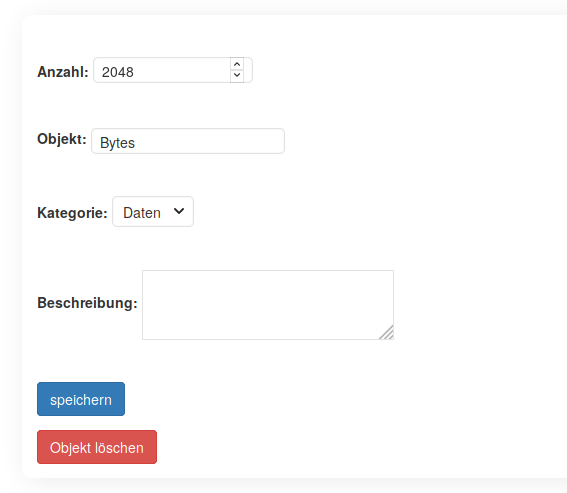
\includegraphics[width=\linewidth]{edit_Obj.png}
So sieht das Fenster zum bearbeiten von Objekten aus.
\end{center}
\subsection{Einstellungen}
Wenn sie in der Navigationsleiste auf den ''Einstellungen'' Button klicken, wird eine Übersicht zum bearbeiten der Nutzereinstellungen angezeigt. Dort können sie ihren Nutzernamen, ihre Emailaddresse und oder ihr Passwort ändern.
\end{document}
